%!TEX root = ../main.tex
\section{Homework \thesection}

\subsection{Domain Operations}
Recall domain operations and geometric transformations discussed in the lecture.
\begin{enumerate}
\item Why do we use homogeneous coordinates?
\item In the 2D rigid transformation matrix
		\[ \begin{pmatrix}
		R & t \\ 0 & 1
		\end{pmatrix}, \]
		rotation is centered at the origin.
		Sometimes we need to rotate a point around another point instead of the origin.
		Assume that	there are two points \(o=(3,5)\) and \(p=(4,2)\) in the 2D plane.
		Write down the transformation matrix \(T\) that rotates \(p\) around \(o\) by \(45^\circ\) clockwise.
\item Implement a similarity transform in Matlab:
		\[T=\begin{pmatrix}
		\frac{\sqrt{3}}{3} & -\frac{1}{3} & 30 \\
		\frac{1}{3} & \frac{\sqrt{3}}{3} & 40 \\
		0 & 0 & 1
		\end{pmatrix}.
		\]
		It's recommended to read through \href{./hw2/2DGeometrixTransformationRecipe.pdf}{\texttt{2D Geometric Transformation Recipe}} before you start coding, especially if you are not very clear how you're going to do this.
		That doc includes the instructions and tips of implementation, which may save you the time to finish this task.
		Choose any image you like as the input image.
		For simplicity, turn the image into gray-scale if it is not.
		Report the original and the output image; include your verbatim in your pdf submission with brief comments.
		Submit your code together with your report.
\end{enumerate}

\subsubsection{Homogeneous coordinates}
Homogeneous coordinates is an extension of Cartesian coordinate (rectangular coordinate).
With this coordinate system, we can write the transformation in the form of matrix multiplication.
Cartesian coordinate can also reach this target, but with restricts.
For example, the projective transformation cannot be described in Cartesian coordinate, but it can be expressed in homogeneous coordinate.\\
Also, it has the property of linearity.
This makes the combination and addition easier than curvilinear coordinates such as spherical or cylindrical coordinates.\\
Last but not the least, homogeneous coordinate is complete in the field of rational numbers \(\mathbb{Q}\), while spherical and cylindrical coordinates always need irrational numbers since \(\pi\) is involved.


\subsubsection{Rotation centered at a non-origin point}
Assume the center of rotation is \((x_0, y_0, 1)^T\).
Then, we can first shift the center of rotation to the origin, then apply the normal rotation, and shift back.
Thus,
\[ \begin{bmatrix}x'\\ y'\\ 1 \end{bmatrix}=R\left(\begin{bmatrix}x\\ y\\ 1 \end{bmatrix}-\begin{bmatrix}x_0\\ y_0\\ 1 \end{bmatrix}\right)+\begin{bmatrix}x_0\\ y_0\\ 1 \end{bmatrix}. \]
Apply the normal rotation matrix and calculate the product,
\[ \begin{bmatrix}x'\\ y'\\ 1 \end{bmatrix}=\begin{bmatrix} \cos\theta & -\sin\theta & 0 \\ \sin\theta & \cos\theta & 0 \\ 0 & 0 & 1 \end{bmatrix}\begin{bmatrix} x-x_0 \\ y-y_0 \\ 0 \end{bmatrix}+\begin{bmatrix}x_0\\ y_0\\ 1 \end{bmatrix}=\begin{bmatrix} x\cos\theta-y\sin\theta+x_0(1-\cos\theta)+y_0\sin\theta \\ x\sin\theta+y\cos\theta-x_0\sin\theta+y_0(1-\cos\theta) \\ 1 \end{bmatrix}. \]
Writing it in the matrix form, we have
\[ \begin{bmatrix}x'\\ y'\\ 1 \end{bmatrix}=\begin{bmatrix} \cos\theta & -\sin\theta & x_0(1-\cos\theta)+y_0\sin\theta &  \\ \sin\theta & \cos\theta & -x_0\sin\theta+y_0(1-\cos\theta) \\ 0 & 0 & 1 \end{bmatrix}\begin{bmatrix}x\\ y\\ 1 \end{bmatrix}. \]
Plug in \((x_0,y_0)=(3,5)\) and \((x,y)=(4,2)\), and \(\theta=-45^\circ\), we obtained the transformation matrix
\[ T=\begin{bmatrix} \frac{\sqrt{2}}{2} & \frac{\sqrt{2}}{2} & 3-4\sqrt{2} \\ -\frac{\sqrt{2}}{2} & \frac{\sqrt{2}}{2} & 5-\sqrt{2} \\ 0 & 0 & 1 \end{bmatrix}. \]

\subsubsection{Similarity transformation}
The code for similarity transformation in natural (Cartesian) coordinate (right-hand rule) is listed below.
The transformation matrix is defined at line 2.
So the image seems to be rotated \(30^\circ\) counter-clockwise.
\lstinputlisting[style=Matlab-editor]{./hw2/problem1/similarity.m}
If we use the coordinate in Matlab style (left-hand rule), then the image will seem to be rotated \(30^\circ\) clockwise.
The code is nearly the same, except some coordinates are shifted.
\lstinputlisting[style=Matlab-editor]{./hw2/problem1/similarity_left_hand_coordinate.m}
The effect is shown in Figure \ref{fig:4}.
\begin{figure}[htbp]
	\centering
	\begin{subfigure}[t]{0.5\textwidth}
	    \centering
		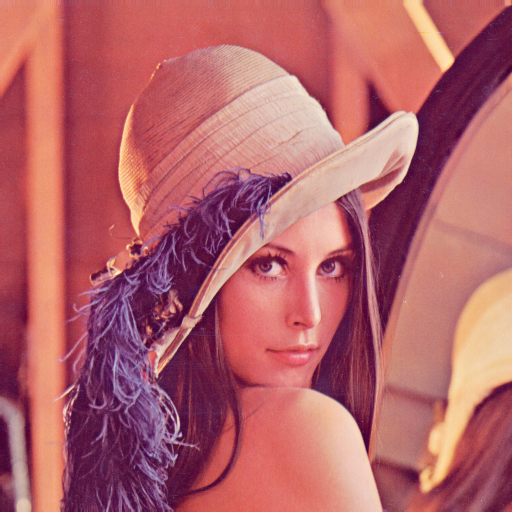
\includegraphics[width=\textwidth]{hw2/problem1/Lenna.png}
		\caption{Original}\label{fig:4a}
	\end{subfigure}\\
	\begin{subfigure}[t]{0.4\textwidth}
	    \centering
		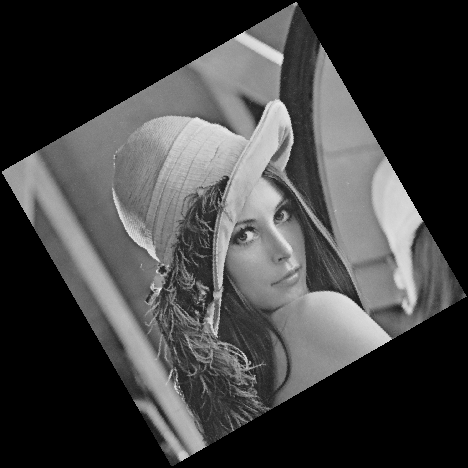
\includegraphics[width=\textwidth]{hw2/problem1/lena.png}
		\caption{Transformation in natural (Cartesian) coordinates (new homework)}\label{fig:4b}
	\end{subfigure}
	\qquad
	\begin{subfigure}[t]{0.4\textwidth}
	    \centering
		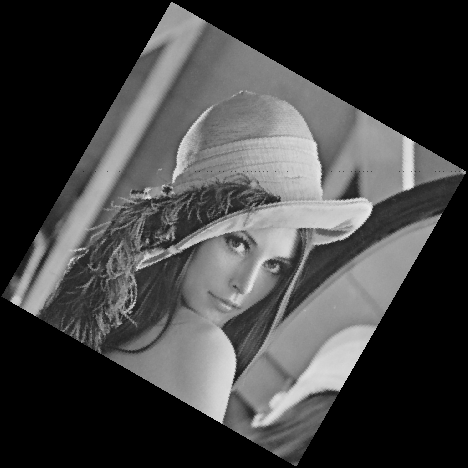
\includegraphics[width=\textwidth]{hw2/problem1/lenal.png}
		\caption{Transformation in Matlab style coordinates (old homework)}\label{fig:4c}
	\end{subfigure}
	\caption{Similarity Transformation}\label{fig:4}
\end{figure}



\newpage


\subsection{3D Structure Tensor}
The Harris operator we discussed at length in lecture computes and analyzes the eigenvalues of the 2D gradient structure tensor (you will implement it below in the third problem).
Let \(\lambda_1\) and \(\lambda_2\) denote the larger and smaller eigenvalues, respectively.
We set two criteria for selection feature points (the value of \(\lambda_2\) and the ratio \(\frac{\lambda_1\lambda_2}{\lambda_1+\lambda_2}\)) based on the analysis of the eigenvalues
(\textit{e.g.}, two small eigenvalues indicate a mostly absent gradient, one large and one small eigenvalue indicate an edge, and two large eigenvalues indicate a corner).\\
Now, consider a video parameterized over \((x,y,t)\in\mathbb{R}^3\).
The eigenvalues of the 3D gradient structure tensor will similarly stratify the pixels in the video into different types.
Let \(\{\lambda_1,\lambda_2,\lambda_3\}\) denote the three eigenvalues of this 3D structure tensor (sorted in decreasing order).
\begin{enumerate}
\item Derive the form of the 3D structure tensor from the SSD error function (for window \(W\)):
		\[ E(u,v,w)=\sum_{u,v,w\in W}\left[\mathcal{I}(x+u,y+v,t+w)-\mathcal{I}(x,y,t) \right]^2 \]
		Propose a criterion to extract ``3D corners''.
\item Answer the question ``What is a 3D corner?''.
		What is an example of a physical phenomenon that may give rise to three large eigenvalues?
		Remember this is space-time and not 3D space, such as that you would image with MRI, for example.
\end{enumerate}


\subsubsection{3D structure tensor derivation}
We apply Taylor's expansion up to first order on \(\mathcal{I}(x+u,y+v,t+w)\):
\[ \mathcal{I}(x+u,y+v,t+w)\approx\mathcal{I}(x,y,t)+\partial_x\mathcal{I}(x,y,t)\cdot u+\partial_y\mathcal{I}(x,y,t)\cdot v+\partial_t\mathcal{I}(x,y,t)\cdot w. \]
Then the SSD error function can be approximated by
\[ E(u,v,w)\approx\sum_{u,v,w\in W}\left(\partial_x\mathcal{I}(x,y,t)\cdot u+\partial_y\mathcal{I}(x,y,t)\cdot v+\partial_t\mathcal{I}(x,y,t)\cdot w\right)^2. \]
For simplicity, denote the partial derivatives as \(\mathcal{I}_x\coloneqq\partial_x\mathcal{I}(x,y,t)\), \(\mathcal{I}_t\coloneqq\partial_t\mathcal{I}(x,y,t)\), \(\mathcal{I}_t\coloneqq\partial_t\mathcal{I}(x,y,t)\), and we obtain the matrix form:
\[ E(u,v,w)\approx\begin{bmatrix} u & v & w \end{bmatrix} \underbrace{\begin{bmatrix} \sum_{u,v,w\in W}\mathcal{I}_x^2 & \sum_{u,v,w\in W}\mathcal{I}_x\mathcal{I}_y & \sum_{u,v,w\in W}\mathcal{I}_x\mathcal{I}_t \\ \sum_{u,v,w\in W}\mathcal{I}_x\mathcal{I}_y & \sum_{u,v,w\in W}\mathcal{I}_y^2 & \sum_{u,v,w\in W}\mathcal{I}_y\mathcal{I}_t \\ \sum_{u,v,w\in W}\mathcal{I}_x\mathcal{I}_t & \sum_{u,v,w\in W}\mathcal{I}_y\mathcal{I}_t & \sum_{u,v,w\in W}\mathcal{I}_t^2 \end{bmatrix}}_\text{3D structure tensor} \begin{bmatrix} u \\ v \\ w \end{bmatrix}. \]
And the matrix in the middle is the 3D structure tensor.
Since the 3D structure tensor is symmetric, its eigenvalues are real.
Furthermore, by construction, it is also positive semi-definite.
Using the analogy of 2D structure tensor, we can propose a criterion to select feature points:
\[ \frac{1}{\frac{1}{\lambda_1}+\frac{1}{\lambda_2}+\frac{1}{\lambda_3}}, \]
which mainly depends on the smallest eigenvalue \(\lambda_3\).
If \(\lambda_3\gg0\), then this value will be large, and will be detected as 3D corner.

\subsubsection{3D corner definition and example}
The 3D corner should be a moving 2D corner on \((x,y)\in\mathbb{R}^2\).
If the corner is static, then \(\mathcal{I}_t=0\), and thus \(\lambda_3=0\), which will not be selected by the criterion.
If the 2D structure is not a corner, then it already has a small eigenvalue, so no matter it is moving or not, it will not be selected as a 3D corner.
An example is a falling box in a static background.
The vertices of the box will be recognized as 3D corners.


\subsection{Local Image Features and Image Stitching}
We motivated and derived an initial local image feature point detector based on an eigendecomposition of the structure tensor.
We also demonstrated an application example of image stitching.
In this question, you will explore these topics further.
\begin{enumerate}
\item Implement the local structure tensor construction and eigendecomposition as described in class.
		This method is called Harris, but implement the simplified corner response measure based on the minimum eigenvalue of the structure tensor, as discussed in class.
		The source file to which you should add code is \href{./hw2/problem3/harris.m}{\texttt{harris.m}}.
		It includes a comment block indicating where you should fill in your code.
		The function should return \texttt{C} where every pixel contains the corner strength.
		This is a ``corner response image''.
		To test your code, you should run \href{./hw2/problem3/run_3_1.m}{\texttt{run\_3\_1.m}}, which will load a simple checkerboard image and execute your harris function on it.
		This will generate two images in figures and save them to disk.
		\href{./hw2/problem3/response_checkerboard.png}{\texttt{response\_checkerboard.png}} is the checkerboard response image (directly from harris) and \href{./hw2/problem3/detect_checkerboard.png}{\texttt{detect\_checkerboard.png}} is the actual corner detections.
		The detect script will run a non-maximal suppression routine and extract corner locations from the response image.\\
		Include two images as well as your code verbatim in the pdf report.
		Submit the \href{./hw2/problem3/harris.m}{\texttt{harris.m}} together with the report.
\item Run the \href{./hw2/problem3/run_3_2.m}{\texttt{run\_3\_2.m}} script; it will load an image of \href{./hw2/problem3/rings.png}{concentric rings} and generate a corner response image \href{./hw2/problem3/response_rings.png}{\texttt{response\_rings.png}}.
		Please discuss the response image explaining why it looks like it does.
		Specifically describe why there are so many responses yet there are no ``corners'' in the image, and why, even though, there are many responses, no full ring has a high corner response over the entire ring.
		Include the image and your response in the writeup.
\item Run the \href{./hw2/problem3/run_3_3.m}{\texttt{run\_3\_3.m}} script.
		It will load the same concentric rings and generate the image that is on the right.
		It is a mess. There are very many false positive corners.
		Figure out a way, any way, that will improve this result to get corners only on the right boundaries at most.
		You can add any code you want to \href{./hw2/problem3/run_3_3.m}{\texttt{run\_3\_3.m}};
		you may change the code that is there.
		You may not call Image Processing Toolbox functions for detecting corners;
		you must use our detectors, but you can change/add to the other parts of the code.
		Remove the false positives so that you only have detected corners on the ring boundaries.
		Include your new \href{./hw2/problem3/run_3_3.m}{\texttt{run\_3\_3.m}} (as `.m' and text in the report) and the best \href{./hw2/problem3/detect_rings.png}{\texttt{detect\_rings.png}} that you can generate.
\item This question will show you an end-to-end use of these computer vision tools by automatically stitching together the left two images below to generate the stitched one on the right.
		No human intervention is needed.
		To make this possible a lot of existing code has been provided to you; your \href{./hw2/problem3/harris.m}{\texttt{harris.m}} is all we additionally need to accomplish this task.\\
		% See for yourself: run \href{./hw2/problem3/run_red.m}{\texttt{run\_red.m}}. Amazing, right?
		The code for doing this has the three basic pieces: reduction (extraction of corners and representation with HOG features), matching (finding the best \texttt{K} correspondences across the images), and estimation (computation of the homography that aligns the two image).
		You can walk through the code to get a better sense of these steps; ask questions if you have them.\\
		Run \href{./hw2/problem3/run_red_varyk.m}{\texttt{run\_red\_varyk.m}}, which will run the whole process three times but vary the number of correspondences that are selected.
		In each run, it will generate some images \href{./hw2/problem3/red_showcorrespondences_K.png}{\texttt{red\_showcorrespondences\_K.png}} and \href{./hw2/problem3/red_stitched1_K.png}{\texttt{red\_stitched1\_K.png}} where \texttt{K} is the number of correspondences (4, 10 or 20).
		The first image shows the extracted correspondences and the second shows the stitching.
		To fit the homography, at least 4 correspondences are needed, which is why we use 4.
		But, 4 seems to yield an inaccurate stitching.
		10 is much better.
		However, when we go to 20, it fails completely.
		Explain
		\begin{enumerate}[(1)]
		\item why 4 correspondences is worse than 10;
		\item why 20 correspondences, which we may expect to be better, completely fails.
		\end{enumerate} 
		Include the six images and your explanations in the report.
		You should use your \href{./hw2/problem3/harris.m}{\texttt{harris.m}} to answer this question.
\end{enumerate}

\subsubsection{Local structure tensor construction and eigendecomposition}
The code of Harris operator implementation is listed here.
\lstinputlisting[style=Matlab-editor]{./hw2/problem3/harris.m}


\begin{figure}[htbp]
	\centering
	\begin{subfigure}[t]{0.3\textwidth}
	    \centering
		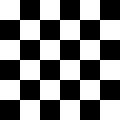
\includegraphics[width=\textwidth]{hw2/problem3/checkerboard.png}
		\caption{Original}\label{fig:5a}
	\end{subfigure}
	\begin{subfigure}[t]{0.3\textwidth}
	    \centering
		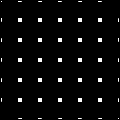
\includegraphics[width=\textwidth]{hw2/problem3/response_checkerboard.png}
		\caption{Response}\label{fig:5b}
	\end{subfigure}
	\begin{subfigure}[t]{0.3\textwidth}
	    \centering
		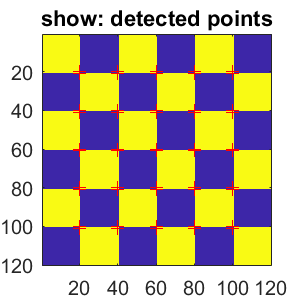
\includegraphics[width=\textwidth]{hw2/problem3/detect_checkerboard.png}
		\caption{Detect}\label{fig:5c}
	\end{subfigure}
	\caption{Corner detection on a checkerboard}\label{fig:5}
\end{figure}

\subsubsection{False positive responses of corners}
All the responses in Figure \ref{fig:6b} are indeed corners.
The reason that we don't regard many of them as corners is that we don't look closely enough.
By zooming in the Figure \ref{fig:6a}, we can see many corners on the ``circles'', since the pixels are discrete so that they cannot form perfect curves.
The only exceptions are 12 o'clock, 3 o'clock, 6 o'clock and 9 o'clock positions of the circles, where the edges are horizontal or vertical, so that the pixels can perfectly form the lines as boundaries.
\begin{figure}[htbp]
	\centering
	\begin{subfigure}[t]{0.4\textwidth}
	    \centering
		
\includegraphics[width=\textwidth]{hw2/problem3/rings.png}
		\caption{\href{./hw2/problem3/rings.png}{\texttt{rings.png}}}\label{fig:6a}
	\end{subfigure}
	\qquad
	\begin{subfigure}[t]{0.4\textwidth}
	    \centering
		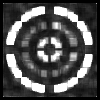
\includegraphics[width=\textwidth]{hw2/problem3/response_rings.png}
		\caption{\href{./hw2/problem3/response_rings.png}{\texttt{response\_rings.png}}}\label{fig:6b}
	\end{subfigure}
	\caption{False positive response example}\label{fig:6}
\end{figure}

\subsubsection{False positives removal}
We decrease the window size to 1, and almost all the detected points lie on the circles, as is shown in Figure \ref{fig:7}.
This is because the window size was too large in the original code.
Since the original graph is noisy, we detected many non-corner points.
By reducing the window size, the Harris operator on each pixel only involves the adjacent pixels, which makes the true corners stand out.
\lstinputlisting[style=Matlab-editor]{./hw2/problem3/run_3_3.m}
\begin{figure}[htbp]
	\centering
	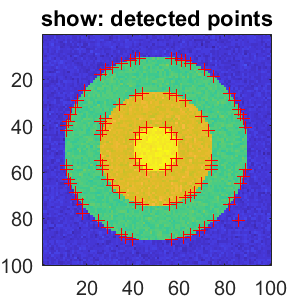
\includegraphics[width=0.95\textwidth]{hw2/problem3/detect_rings.png}
	\caption{False positive response removal}\label{fig:7}
\end{figure}



\subsubsection{Image stitching}
The projection transform matrix has 8 degrees of freedom, and 4 matching points has exactly 8 coordinates, so the 8 free entries in the projection transform matrix are uniquely determined.
However, each matching point might not be determined accurately, so the projection transform matrix is not accurate.
When 10 matching points are selected, 20 coordinates are generated to determine the 8 free entries of the projection transform matrix.
Thus, there are redundancy in the coefficients, and Linear Least Square method is applied to determine the best projection transform matrix.
Although all the 20 coordinates contain some random error, they cancel out when least square method is applied.

On the other hand, when 20 matching points are selected, many of them are not actually matching.
Particularly, the two images have many local features that are very similar, but not matching points.
For example, the crossings on the windows are the most deceptive features.
Many crossings on the left window in image 1 are matched to the crossings on the right window in image 2, while they are not the same points on the actual building.
The \href{./hw2/problem3/match.m}{\texttt{match.m}} script uses a sorting algorithm to sort the matching pairs of points, so if the top 10 are picked, no false matching are selected, but when 20 points are selected, the 11\(^\text{th}\) to 20\(^\text{th}\) pairs contains many false matching.
In Figure \ref{fig:9b}, the rightmost two pillars in image 1 are matched to the leftmost two pillars in image 2, which is correct.
But in Figure \ref{fig:9c}, the pillar in the center in image 1 is matched to the middle pillar in image 2, which is incorrect.
Furthermore, the errors brought by the false matching pairs are much larger than the random errors in true matching pairs, so the LLS method will be influenced by a lot.
Again, LLS method does not ignore the false matching pairs automatically, so the projection transform matrix generated by 20 pairs of matching points are screwed by the false matching points.

\begin{figure}[htbp]
	\centering
	\begin{subfigure}[t]{0.4\textwidth}
	    \centering
		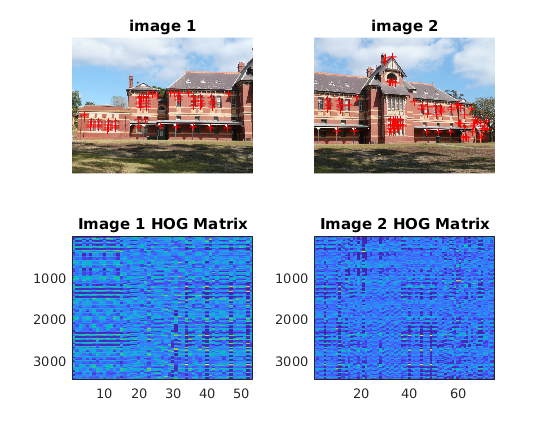
\includegraphics[width=\textwidth]{hw2/problem3/red_showcorrespondences_4.png}
		\caption{\href{./hw2/problem3/red_showcorrespondences_4.png}{\texttt{red\_showcorrespondences\_4.png}}}\label{fig:8a}
	\end{subfigure}
	\qquad
	\begin{subfigure}[t]{0.4\textwidth}
	    \centering
		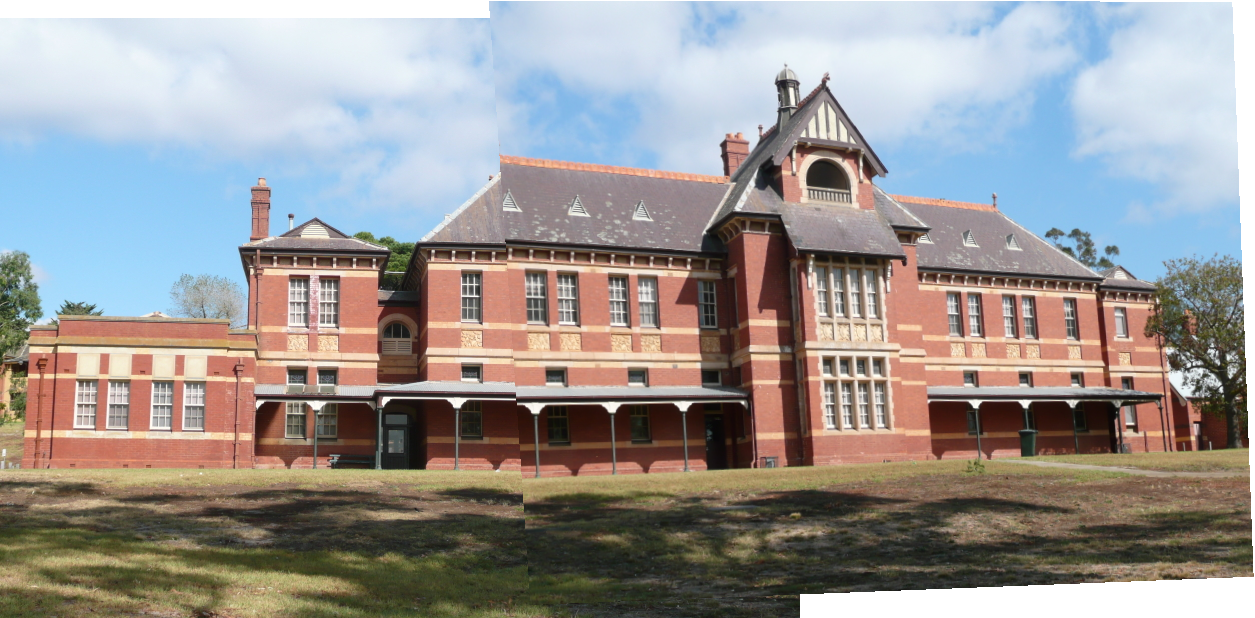
\includegraphics[width=\textwidth]{hw2/problem3/red_stitched1_4.png}
		\caption{\href{./hw2/problem3/red_stitched1_4.png}{\texttt{red\_stitched1\_4.png}}}\label{fig:8b}
	\end{subfigure}
	\begin{subfigure}[t]{0.4\textwidth}
	    \centering
		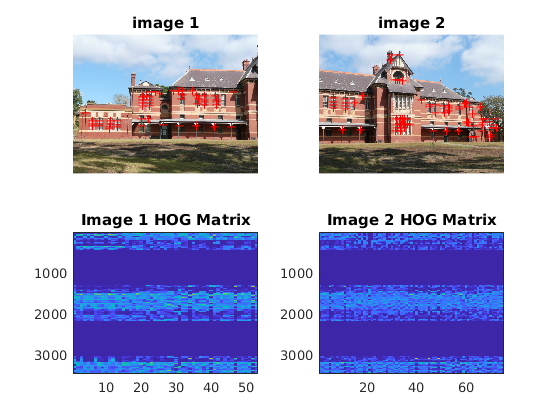
\includegraphics[width=\textwidth]{hw2/problem3/red_showcorrespondences_10.png}
		\caption{\href{./hw2/problem3/red_showcorrespondences_10.png}{\texttt{red\_showcorrespondences\_10.png}}}\label{fig:8c}
	\end{subfigure}
	\qquad
	\begin{subfigure}[t]{0.4\textwidth}
	    \centering
		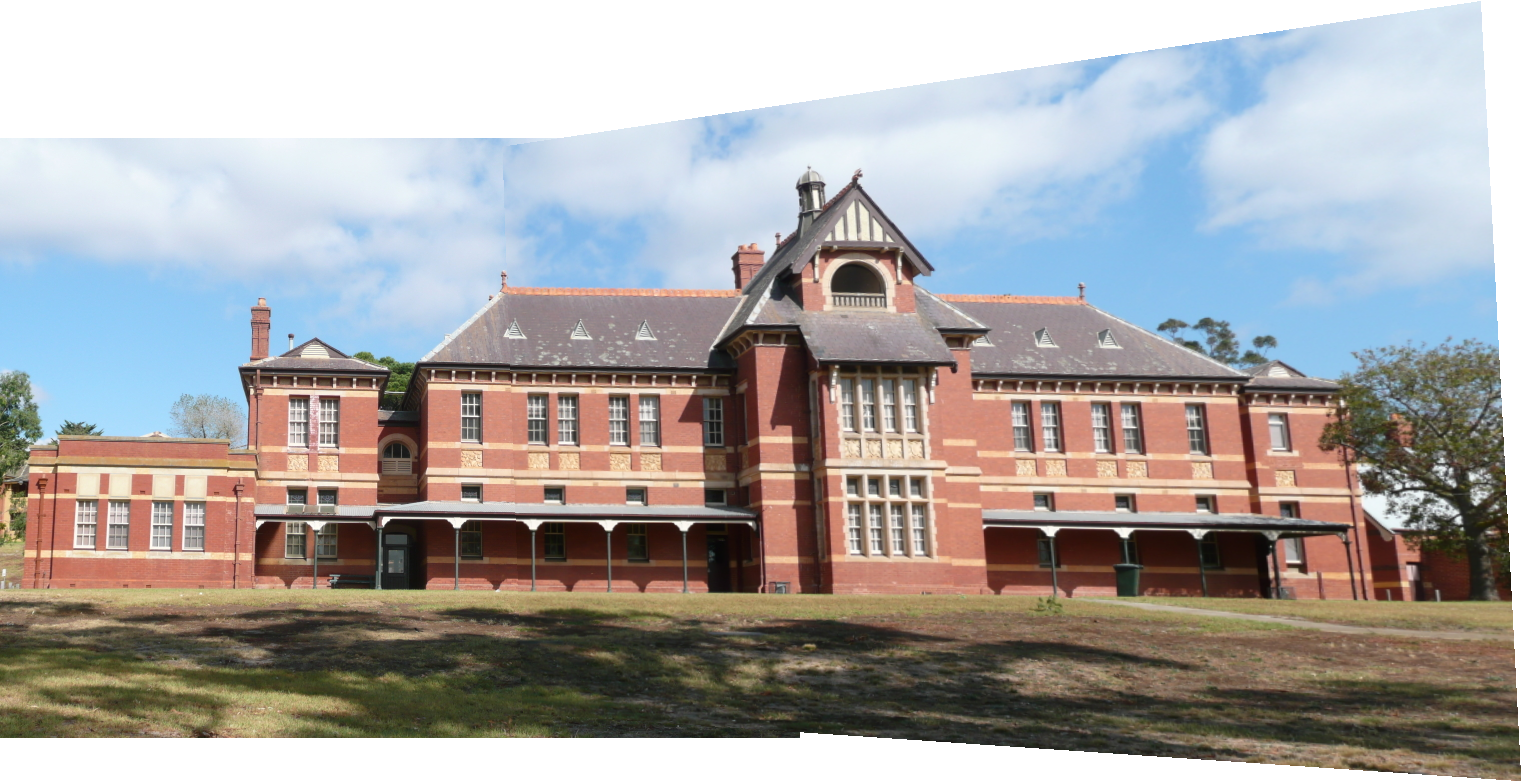
\includegraphics[width=\textwidth]{hw2/problem3/red_stitched1_10.png}
		\caption{\href{./hw2/problem3/red_stitched1_10.png}{\texttt{red\_stitched1\_10.png}}}\label{fig:8d}
	\end{subfigure}
	\begin{subfigure}[t]{0.4\textwidth}
	    \centering
		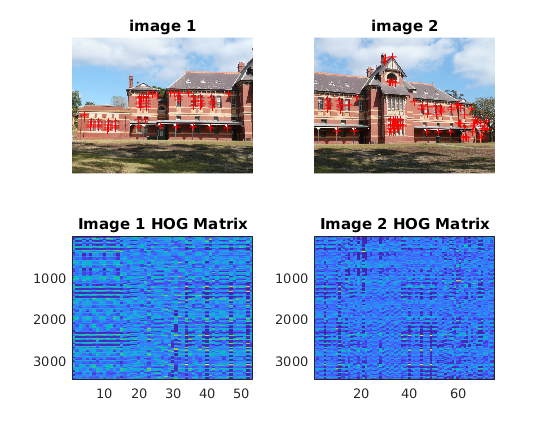
\includegraphics[width=\textwidth]{hw2/problem3/red_showcorrespondences_20.png}
		\caption{\href{./hw2/problem3/red_showcorrespondences_20.png}{\texttt{red\_showcorrespondences\_20.png}}}\label{fig:8e}
	\end{subfigure}
	\qquad
	\begin{subfigure}[t]{0.4\textwidth}
	    \centering
		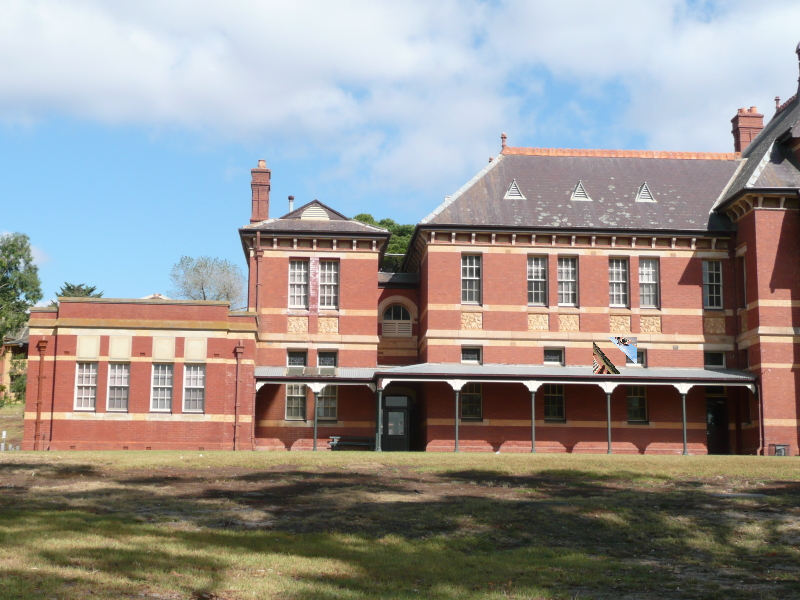
\includegraphics[width=\textwidth]{hw2/problem3/red_stitched1_20.png}
		\caption{\href{./hw2/problem3/red_stitched1_20.png}{\texttt{red\_stitched1\_20.png}}}\label{fig:8f}
	\end{subfigure}
	\caption{Image stitching}\label{fig:8}
\end{figure}


\begin{figure}
	\centering
	\begin{subfigure}[t]{0.7\textwidth}
	    \centering
		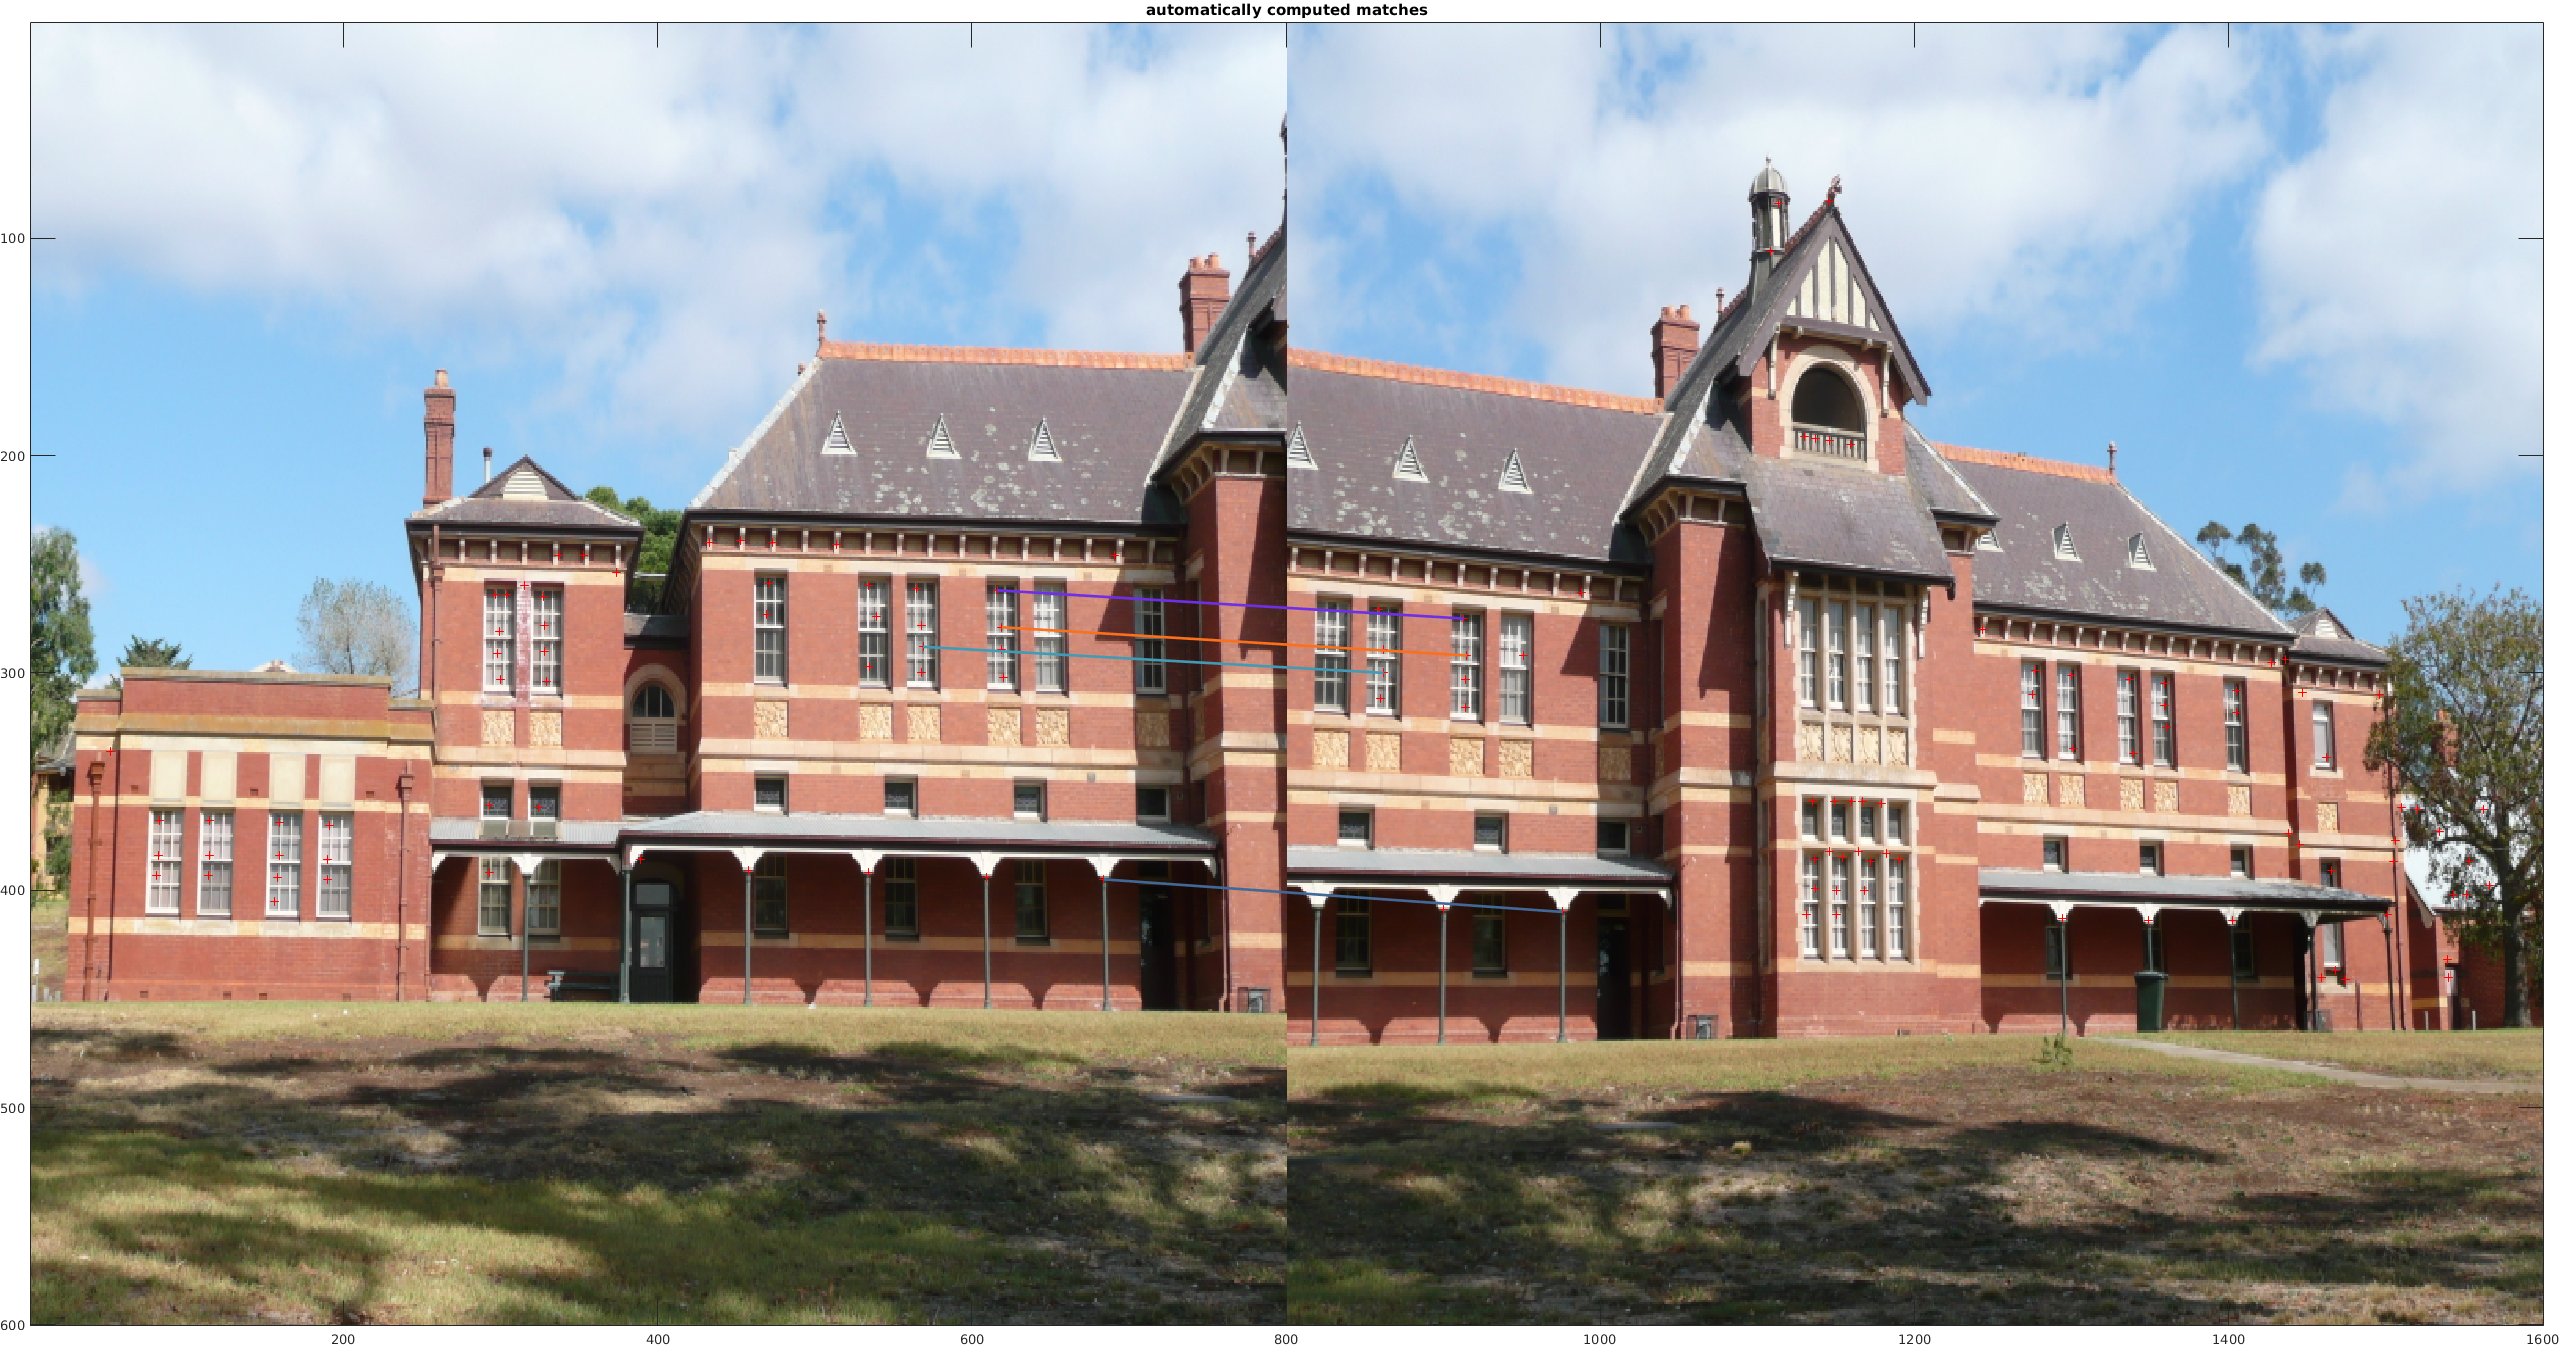
\includegraphics[width=\textwidth]{hw2/problem3/match_4.png}
		\caption{\href{./hw2/problem3/match_4.png}{Match 4}}\label{fig:9a}
	\end{subfigure}
	\begin{subfigure}[t]{0.7\textwidth}
	    \centering
		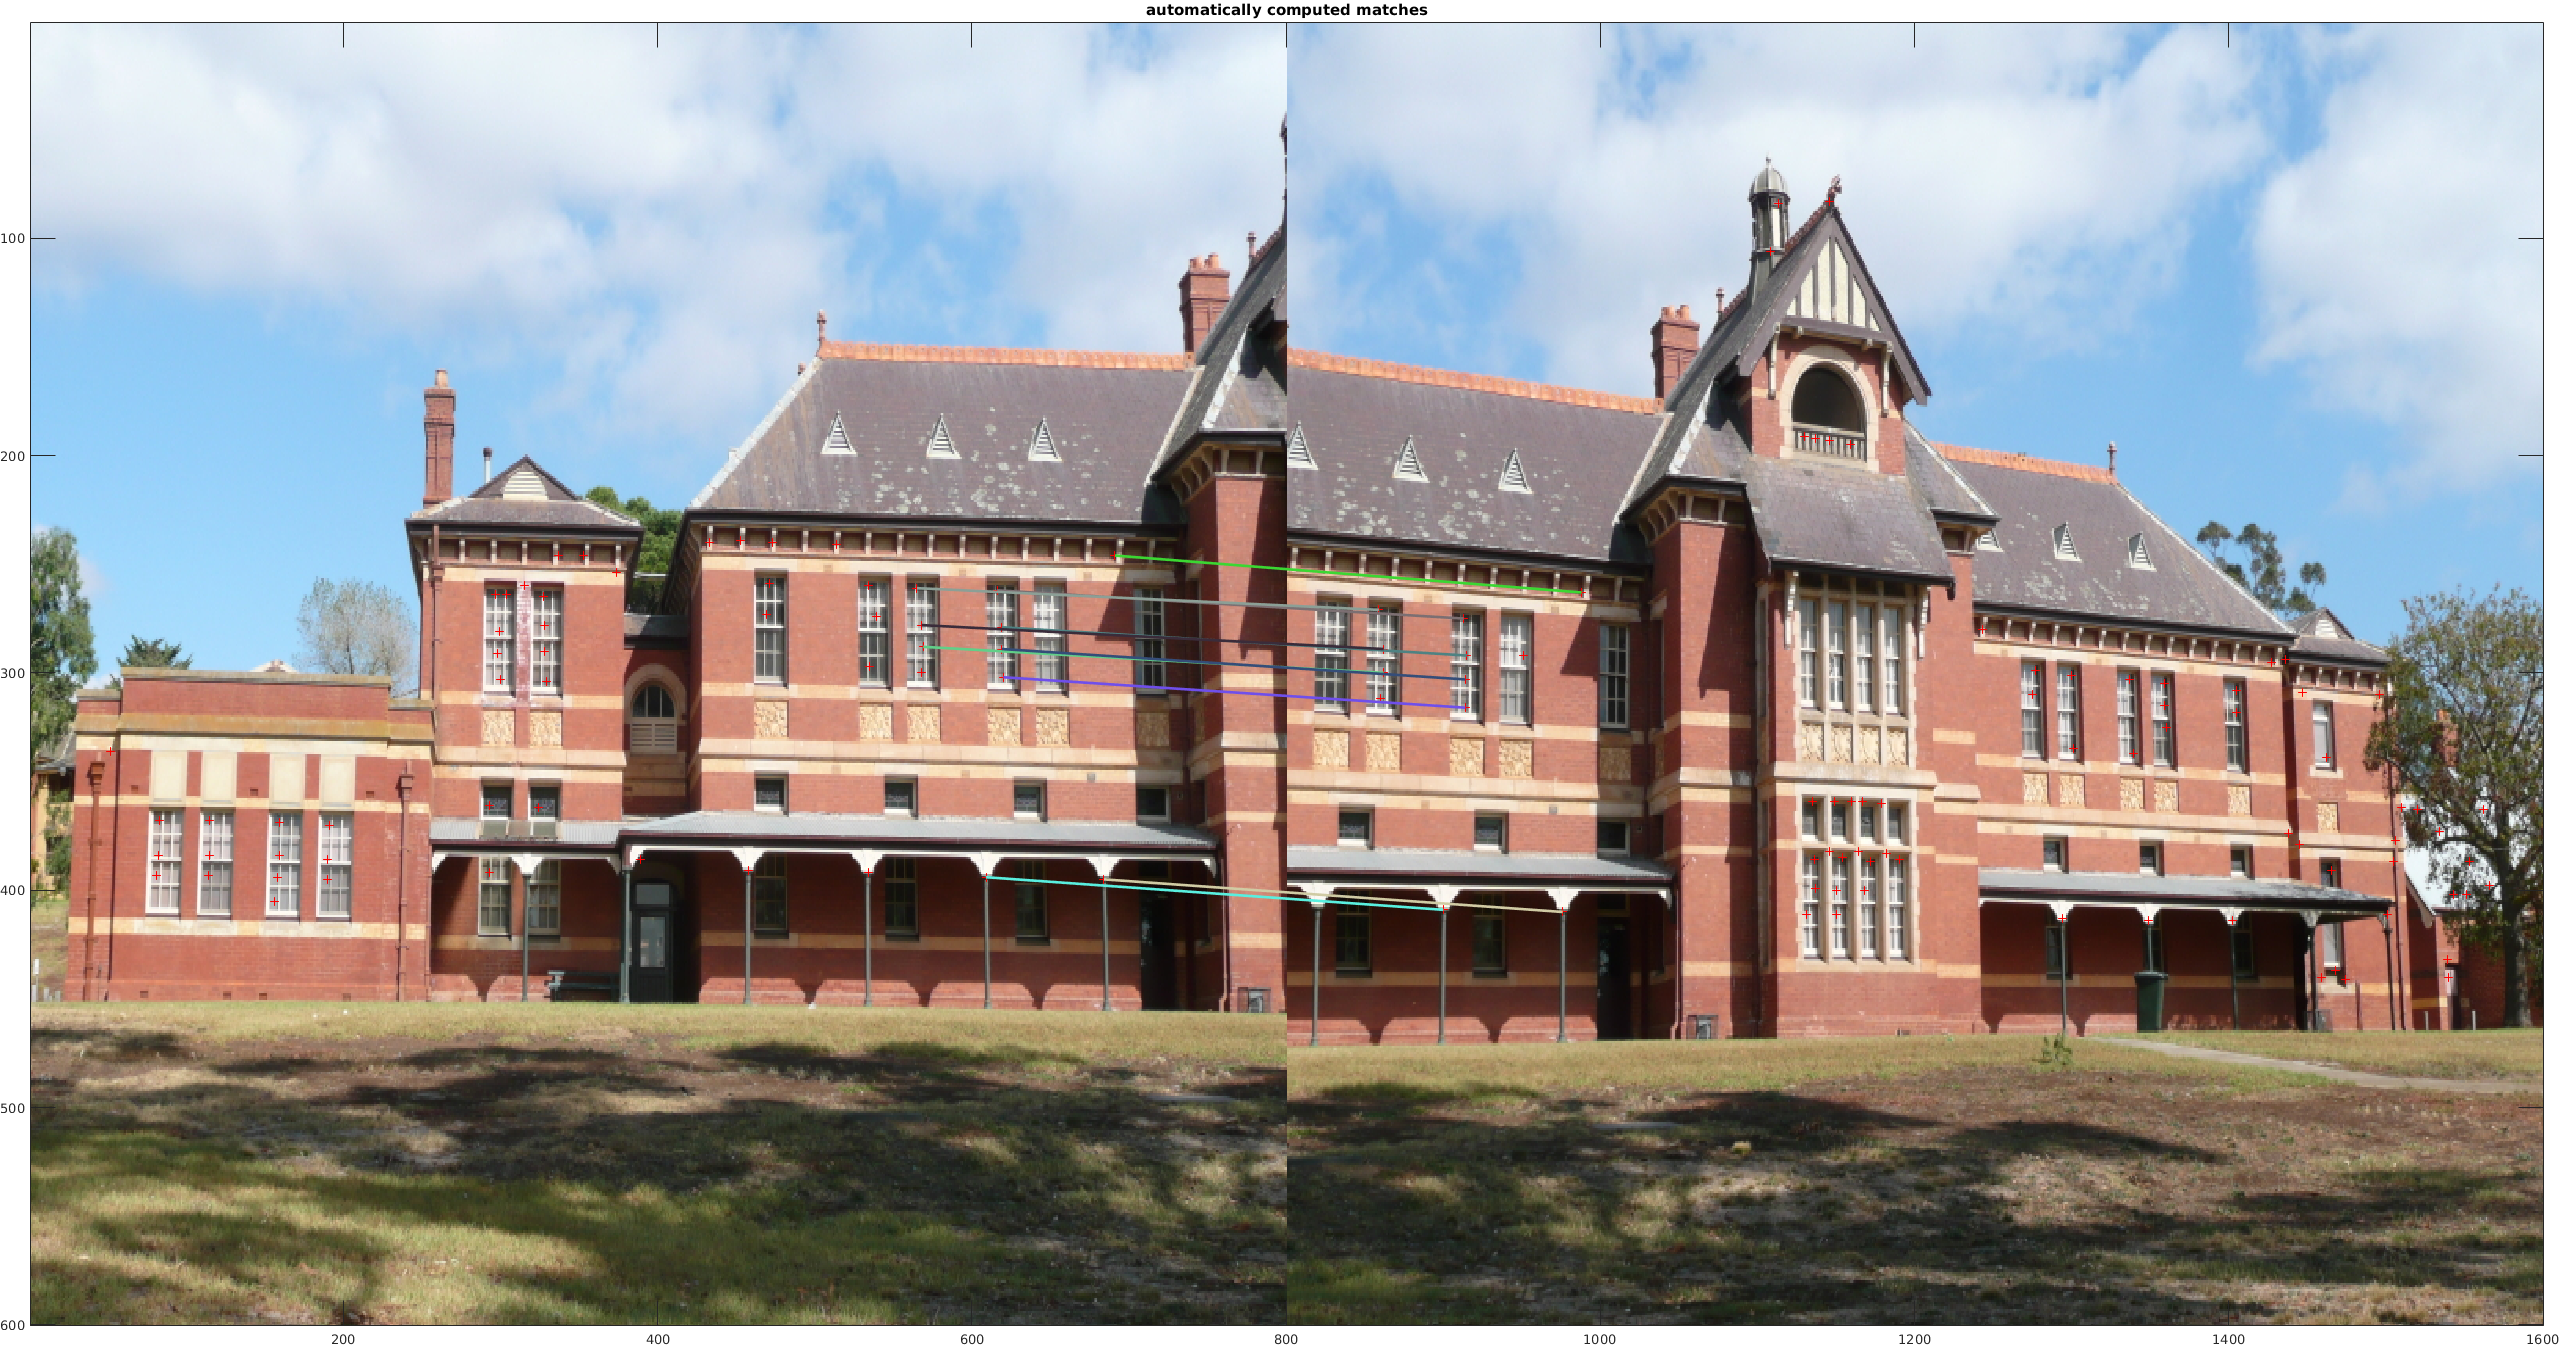
\includegraphics[width=\textwidth]{hw2/problem3/match_10.png}
		\caption{\href{./hw2/problem3/match_10.png}{Match 10}}\label{fig:9b}
	\end{subfigure}
	\begin{subfigure}[t]{0.7\textwidth}
	    \centering
		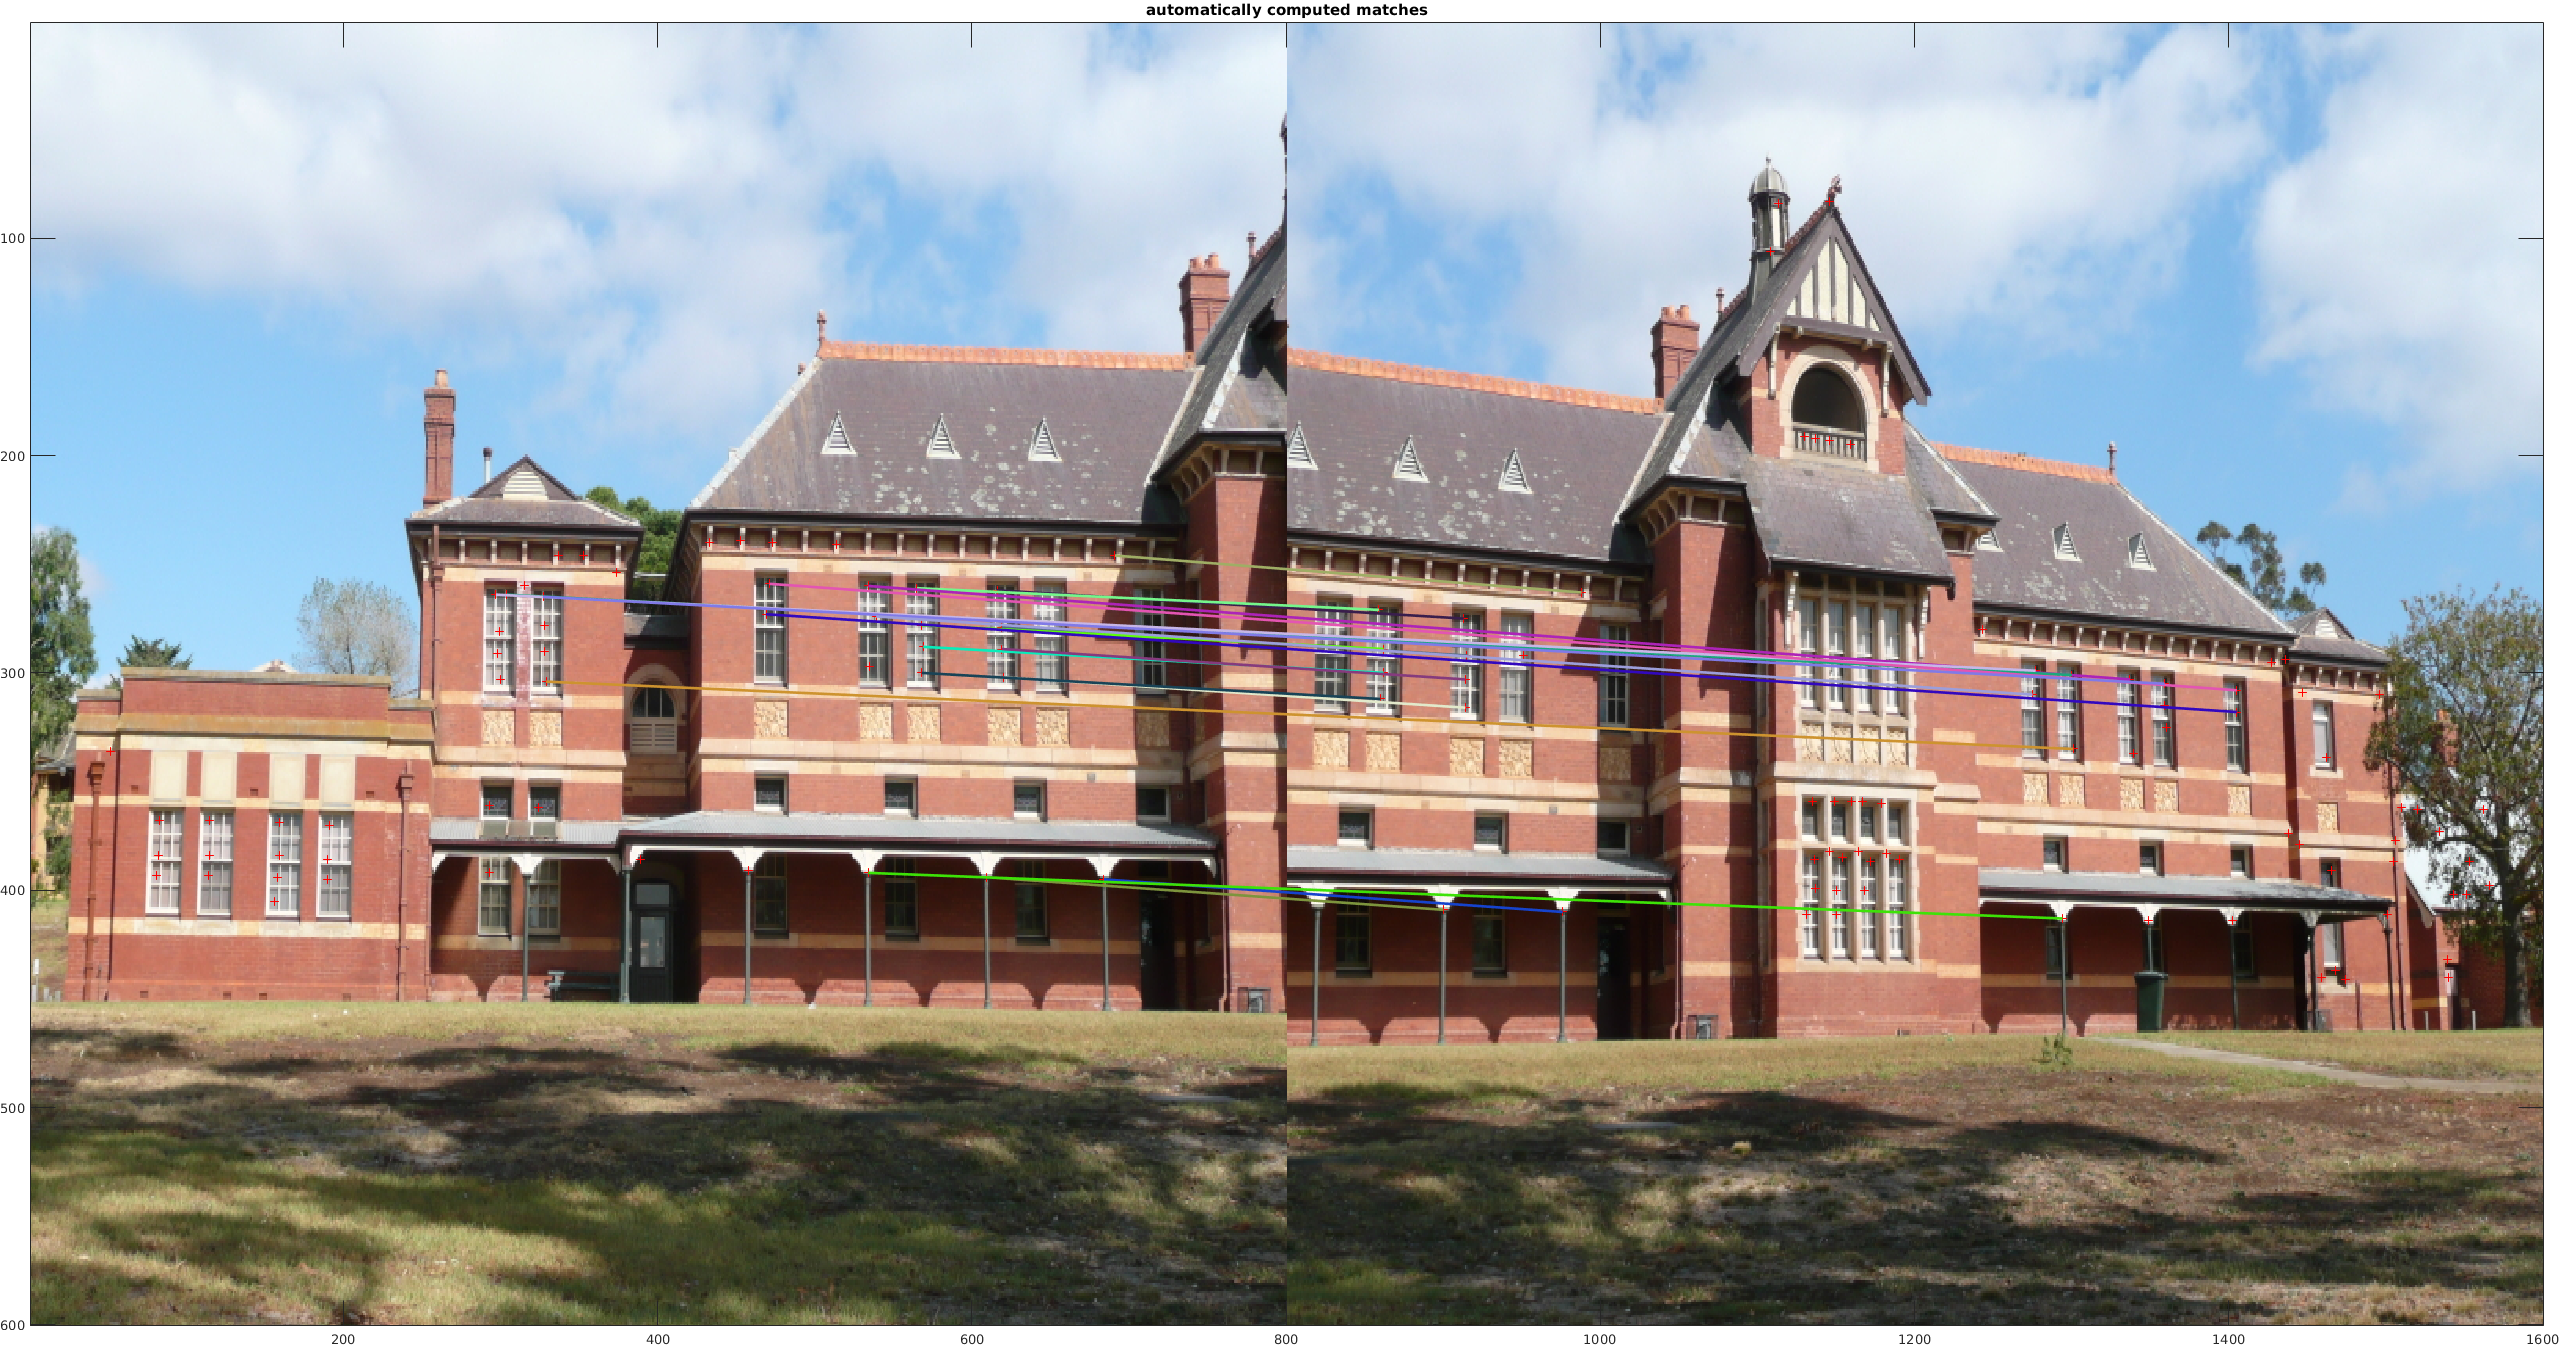
\includegraphics[width=\textwidth]{hw2/problem3/match_20.png}
		\caption{\href{./hw2/problem3/match_20.png}{Match 20}}\label{fig:9c}
	\end{subfigure}
	\caption{Feature points matching}\label{fig:9}
\end{figure}